


Let X and Y be a random variable which takes values from set A and B respectively.We want to calculate Pr(X+Y=16)
\begin{equation}
  p_X(n)=\begin{cases}
    \dfrac{1}{4}, & \text{if } 2\leq n\leq 5.\\
    0, & \text{otherwise}.
  \end{cases}
\end{equation}
\begin{equation}
  p_Y(n)=\begin{cases}
    \dfrac{1}{5}, & \text{if } 11\leq n\leq 15.\\
    0, & \text{otherwise}.
  \end{cases}
\end{equation}
\begin{align}
&p_z(n) = \Pr(X+Y = n) = \Pr(Y=n-X)\\
&p_z(n) = \sum_k p_x(k)p_y(n-k) = p_x(n) * p_y(n)\\
&p_z(n) = \frac{1}{4} \sum_{k=2}^5 p_y(n-k)=\frac{1}{4}\sum_{k=n-5}^{n-2} p_y(k)
\end{align}
\begin{equation}
  p_z(n)=\begin{cases}
  &0 , n < 13\\
  &\dfrac{1}{20}\times (n-12) ,13 \leq n < 16\vspace{0.2cm}\\
  &\dfrac{1}{20} \times 4 , 16 \leq n \leq 17\vspace{0.2cm}\\
  &\dfrac{21-n}{20} , 18 \leq n \leq 20\vspace{0.2cm}\\
  & 0 ,n > 20
  \end{cases}
\end{equation}
\begin{align}
\therefore p_z(16) = \frac{1}{5}
\end{align}
\begin{figure}[h]
    \centering
    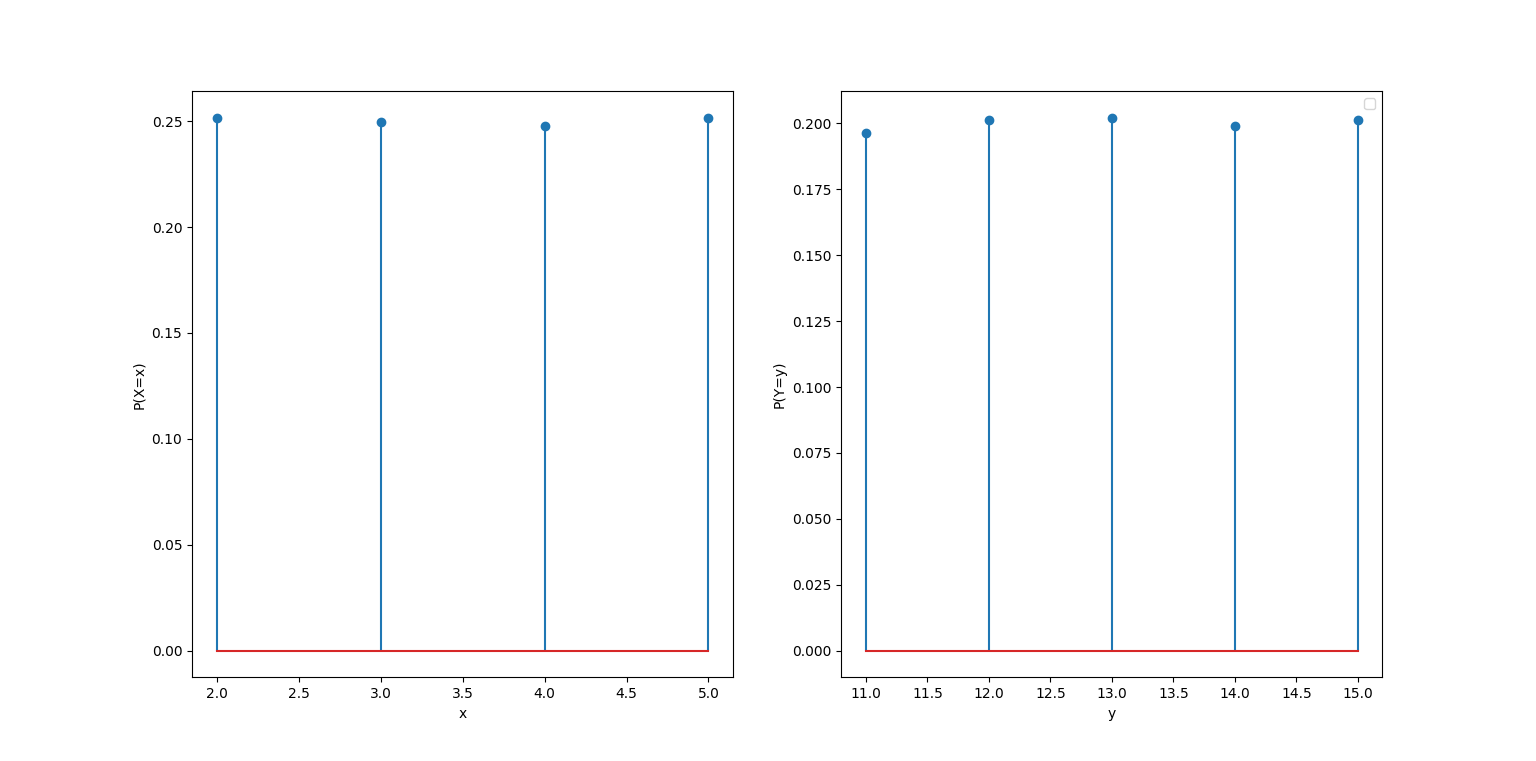
\includegraphics[width=\columnwidth]{solutions/cs/2015/3/figures/assignment4_plot2.png}
\end{figure}
\begin{figure}[h]
    \centering
    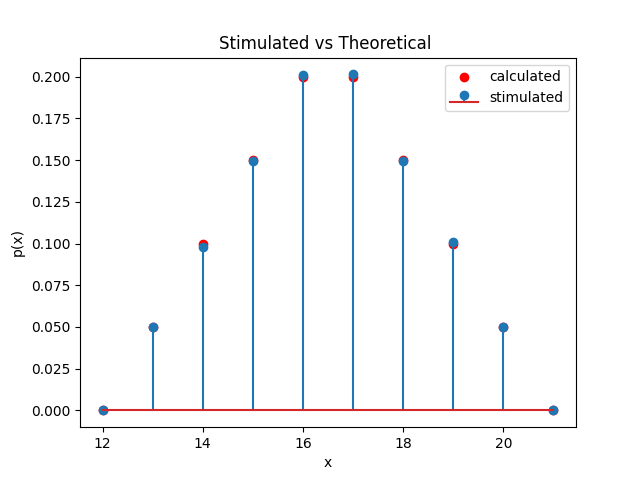
\includegraphics[width=\columnwidth]{solutions/cs/2015/3/figures/assignment4_plot1.png}
\end{figure}

